% AIIT Bulletin Template Version 18.0 2024-07-09; Equivalent Word template version: 6
\documentclass[fontsize=9pt, jafontscale=.95, twocolumn, a4paper]{jlreq}
\usepackage{variables}
\title{東京都立産業技術大学院大学研究紀要執筆ガイド: \YEAR 年度版}
\newcommand{\entitle}{Preperation of papers for the Bulletin of Advanced Instutitue of Industrial Technology: \YEAR}
\author[1*]{松井 実}
\author[1,2]{執筆者 共同}
\author[2,3]{執筆者 最終}
\author[1*]{\authorcr\small Minoru Matsui} % add \authorcr at the beginning of the first author's latin name
\author[1,2]{\small Kyodo Shippitsusha}
\author[2,3]{\small Saishu Shippitsusha}
\affil[1]{東京都立産業技術大学院大学  Advanced Institute of Industrial Technology}
\affil[2]{東京都立大学  Tokyo Metropolitan University}
\affil[3]{東京都立産業技術高等専門学校 Tokyo Metropolitan College of Industrial Technology}
\affil[*]{Corresponding author: Minoru Matsui, xerroxcopy@gmail.com}
\newcommand{\abstractcontent}{Write in English. Lorem ipsum dolor sit amet, consectetur adipiscing elit. Suspendisse ac enim turpis. Morbi eu maximus velit, ac maximus enim. Phasellus et pellentesque ante. Pellentesque non velit id tortor rutrum pretium a ac neque. Sed congue sit amet leo vel laoreet. Vivamus ullamcorper a dolor in aliquet. Pellentesque finibus at nunc ac egestas. Proin eu sollicitudin nisi. Sed cursus pulvinar leo. In erat erat, molestie ac euismod at, egestas non neque. Nam viverra nunc erat, vitae elementum tortor cursus et. Duis sed magna vel turpis congue finibus.Morbi pulvinar auctor quam eget commodo. Quisque mi nulla, tempor quis sem sed, auctor pharetra turpis. Cras blandit vestibulum dapibus. Sed ac nisi et metus sollicitudin tincidunt rutrum eget felis. Donec imperdiet dolor nec elit interdum, vitae ultrices turpis consectetur. Sed lacinia tempus lacinia. Morbi facilisis metus ac diam sollicitudin, et ornare urna rutrum. Nullam sollicitudin fringilla ipsum, nec vulputate risus. Sed sit amet euismod nulla.Proin porttitor diam ac lacus vehicula facilisis. Sed at tempus magna. Aenean eget vehicula ipsum, non porta arcu. Suspendisse vitae lacinia leo. Ut sit amet purus imperdiet ipsum tempor efficitur auctor eget magna. Phasellus suscipit risus eu semper eleifend. Ut tempor magna viverra urna condimentum, sed pretium ipsum iaculis. Pellentesque aliquet tincidunt felis ac imperdiet.Phasellus viverra tristique lorem, in dignissim risus bibendum non. Praesent varius urna eget nibh lacinia, sed faucibus turpis tristique. Proin hendrerit pretium ullamcorper . Donec non vestibulum diam. Sed suscipit, justo sit amet auctor aliquam, orci sem sollicitudin lacus, et maximus. (max 250 words)}
\newcommand{\keywordscontent}{keyword1; keyword2; keyword3 (max 5 keywords)}
% \newcommand{\doi}{10.1000/aiit0017}
% import a package set
\usepackage{aiit}

% load settings for layouts and aesthetic tweaks. 
% comment this out to speed up compile (draft quality)
\usepackage{aiit-aes} 

\begin{document}
\twocolumn[%

\vspace{-15mm}
\maketitle
\vspace{-8mm}
\begin{spacing}{.8}
% \begin{onecolabstract}
\begin{abstract}
\abstractcontent
\end{abstract}
% \end{onecolabstract}
\small\textbf{Keywords\quad}\keywordscontent\\
\vspace{2mm}
\rule{\textwidth}{.1mm}
\end{spacing}
\vspace{8mm}
]
\pagestyle{aiit}
\section{はじめに}

本稿では、東京都立産業技術大学院大学研究紀要の執筆用LaTeXテンプレート(日本語版\cite{Matsui2024-lk};英語版\cite{Matsui2024-vp})について記す(本紀要執筆ガイドは\YEAR 年度版)。編集委員は提出された原稿をチェックはするが、体裁を整えることはしないので、無編集で公開しても問題ない品質に仕上げるための方法を説明する。

原稿は、日本語もしくは英語による完全版下 (camera ready) 原稿とする。製版後の校正は原則として不可能であるため、誤字や脱字がないよう、特に念を入れて仕上げる。刷り上がりは6ページ以上が望ましい。余白や段組、使用するフォントやフォントサイズを変更せず、そうしなければ論文としての体裁が整わないのでない限りこのテンプレートファイルに用意されたスタイルのまま仕上げる。

\subsection*{環境}

コンパイラにはLuaLaTeXを使用し、\verb|main.tex|をコンパイルする。\verb|aiit.sty|は記述に必須のパッケージが入っているので常に\mintinline{latex}{\usepackage{aiit}}としてインポートするべきだが、\verb|aiit-aes.sty|はレイアウトやヘッダー・フッターのスタイリングなどに関する設定が入っているため、下書きの段階では\mintinline{latex}{\usepackage{aiit-aes}}の行はコメントアウトしておいてもよい(コンパイルが少し早くなる)。TeX Liveのバージョンは2024を想定している。クラウド上でTeX文書を編集・生成できるサービスOverleafでの利用を想定している。Overleafを利用する場合、無料版の契約では制限時間内に\YEAR 年度現在の本テンプレートのコンパイルが終わらないため、有料版を契約する必要がある。自らの責任においてCloud LaTeXやローカル環境で使用してもよい。後述するmintedパッケージはPygmentsを使用するため、Overleaf以外の環境で本テンプレートを使用する場合はPygmentsをインストールするか、mintedに関連する記述を削除し、デフォルトの\verb|\verb|や\verb|\verbatim|を用いる。

\section{表題、著者名、概要}

\subsection*{表題}

表題は\mintinline{latex}{\title{}}の中に、副題は題のあとに: に続けて表記する。表題の英訳は\verb|main.tex|内の\mintinline{latex}{\newcommand{\entitle}{Title of the paper: subtitle here}}にSentence caseで記述する。

\subsection*{著者名}

著者名はauthblkパッケージを用いて以下の要領で記述する。ローマ字表記には原則としてパスポート表記と同様のヘボン式を用いる(例:ItouでもItōでもなくIto、SenoでもSenōでもなくSenoo)。所属が複数ある場合は番号を半角コンマで区切って表記し、番号の間には半角スペースを入れない。責任著者の連絡先は番号付きの所属と同様に記述し、記号には番号ではなく*を用いる。“Corresponding author: [First name] [Family name], [メールアドレス]”として表記する。コロンのあとや半角カッコのまえに半角スペースを挿入すること。原則として責任著者が退職・修了後も連絡がとれるように少なくとも今後10年間は受信できる予定のメールアドレスを記述する。

\begin{minted}{latex}
\author[`所属を表す肩付き文字`]{`著者の氏` `名`}
\author[`所属を表す肩付き文字`]{\authorcr \small `著者の氏ローマ字表記` `筆頭著者の名ローマ字表記`}

\affil[`肩付き文字`]{\footnotesize `所属の和文表記`  `所属の欧文表記`}
\affil[*]{\footnotesize Corresponding author: `責任著者の氏ローマ字表記` `責任著者の名ローマ字表記`, `責任著者のメールアドレス`}
\end{minted}

\subsection*{概要・キーワード}

論文の概要文は\mintinline{latex}{\newcommand{\abstractcontent}{abstract here}}に英語で250語以下で記述する。英語は米国英語でも英国英語でも構わないが、どちらかに統一する。イタリック体以外の太字・下線・複雑な数式・参考文献の引用は不可。著者全員の責任において破綻のない英文を作成すること。

キーワードは概要の直後の\mintinline{latex}{\newcommand{\keywordscontent}{keywords here}}に記述する。キーワードはlower caseで記述(Keyword; Keywordではなくkeyword; keyword)し、セミコロン(;)で区切る。

% DOIは各論文に割り振られたものを\mintinline{latex}{\newcommand{\doi}{10.1000/aiit0017}}の行に記述する。

\section{本文の編集}

日本語中のかっこは全角かっこ()を、英語中のかっこは半角スペースに囲まれた半角かっこ () を用いる。単位と数値のあいだには半角スペースを追加する。ルビは\ltjruby{東京|都立|産業|技術|大学院|大学|研究|紀要}{とうきょう|とりつ|さんぎょう|ぎじゅつ|だいがくいん|だいがく|けんきゅう|きよう}のようにふることができる。

\subsection*{見出し}

研究紀要は大学に所属する教員や学生が研究内容を対外的に簡潔に発信するためにある。そのため、複数のトピックを扱う学位論文のような媒体でしばしば見られる1.1.1.1のような細分化された見出しは不要である。最も大きい見出しである章には\mintinline{latex}{\section{title here}}を、節には番号をふらない\mintinline{latex}{\subsection*{title here}}を適用する。内容が簡潔であれば節に細分化せず、章のみで記述しても問題はない。

\subsection*{句読点}

和文の句読点には、全角ピリオド(.)と全角コンマ(,)の組み合わせ、もしくは「、。」の組み合わせを用いる。どちらを利用してもよいが、どちらかに統一し、スタイルが混在してはならない。また、英文の句読点には半角ピリオドと半角スペース(. )、半角コンマと半角スペース(, )を用いること。

\section{図表、コード、数式}

\subsection*{図}

図は小さいものであれば図\ref{figure:figureExample}のように1カラムいっぱいの幅(86 mm)で出力し、大きいものは図\ref{figure:figureExampleLarge}のように余白を除いた紙面いっぱいの幅(186 mm)で出力する。\verb|\label|は\verb|\caption|の直後に記述する。

図の品質は印刷に十分耐えうるものでなければならない。刷り上がり時の文字が小さすぎないよう十二分に配慮し、線の太さにも注意する。また、図表の余白にも注意する。図の具体的な描画方法については規定しないが、軸や目盛り線の太さは0.15 mmを推奨し、パネルキャプションや凡例、軸名、数値ラベルなどのフォントサイズは6 ptを推奨する。

\begin{figure}[hbt!]
  \centering
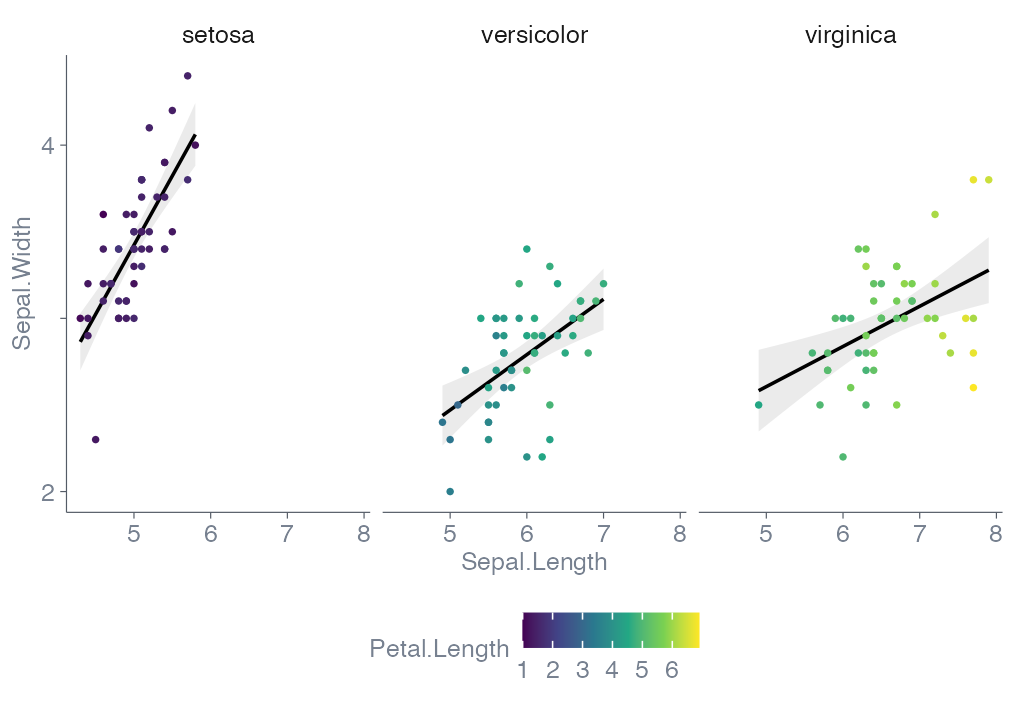
\includegraphics[width=89mm]{p_plot}
    \caption{1カラムの横幅89 mmサイズの図の例。}
    \label{figure:figureExample}
\end{figure}
\begin{figure*}[hbt!]
  \centering
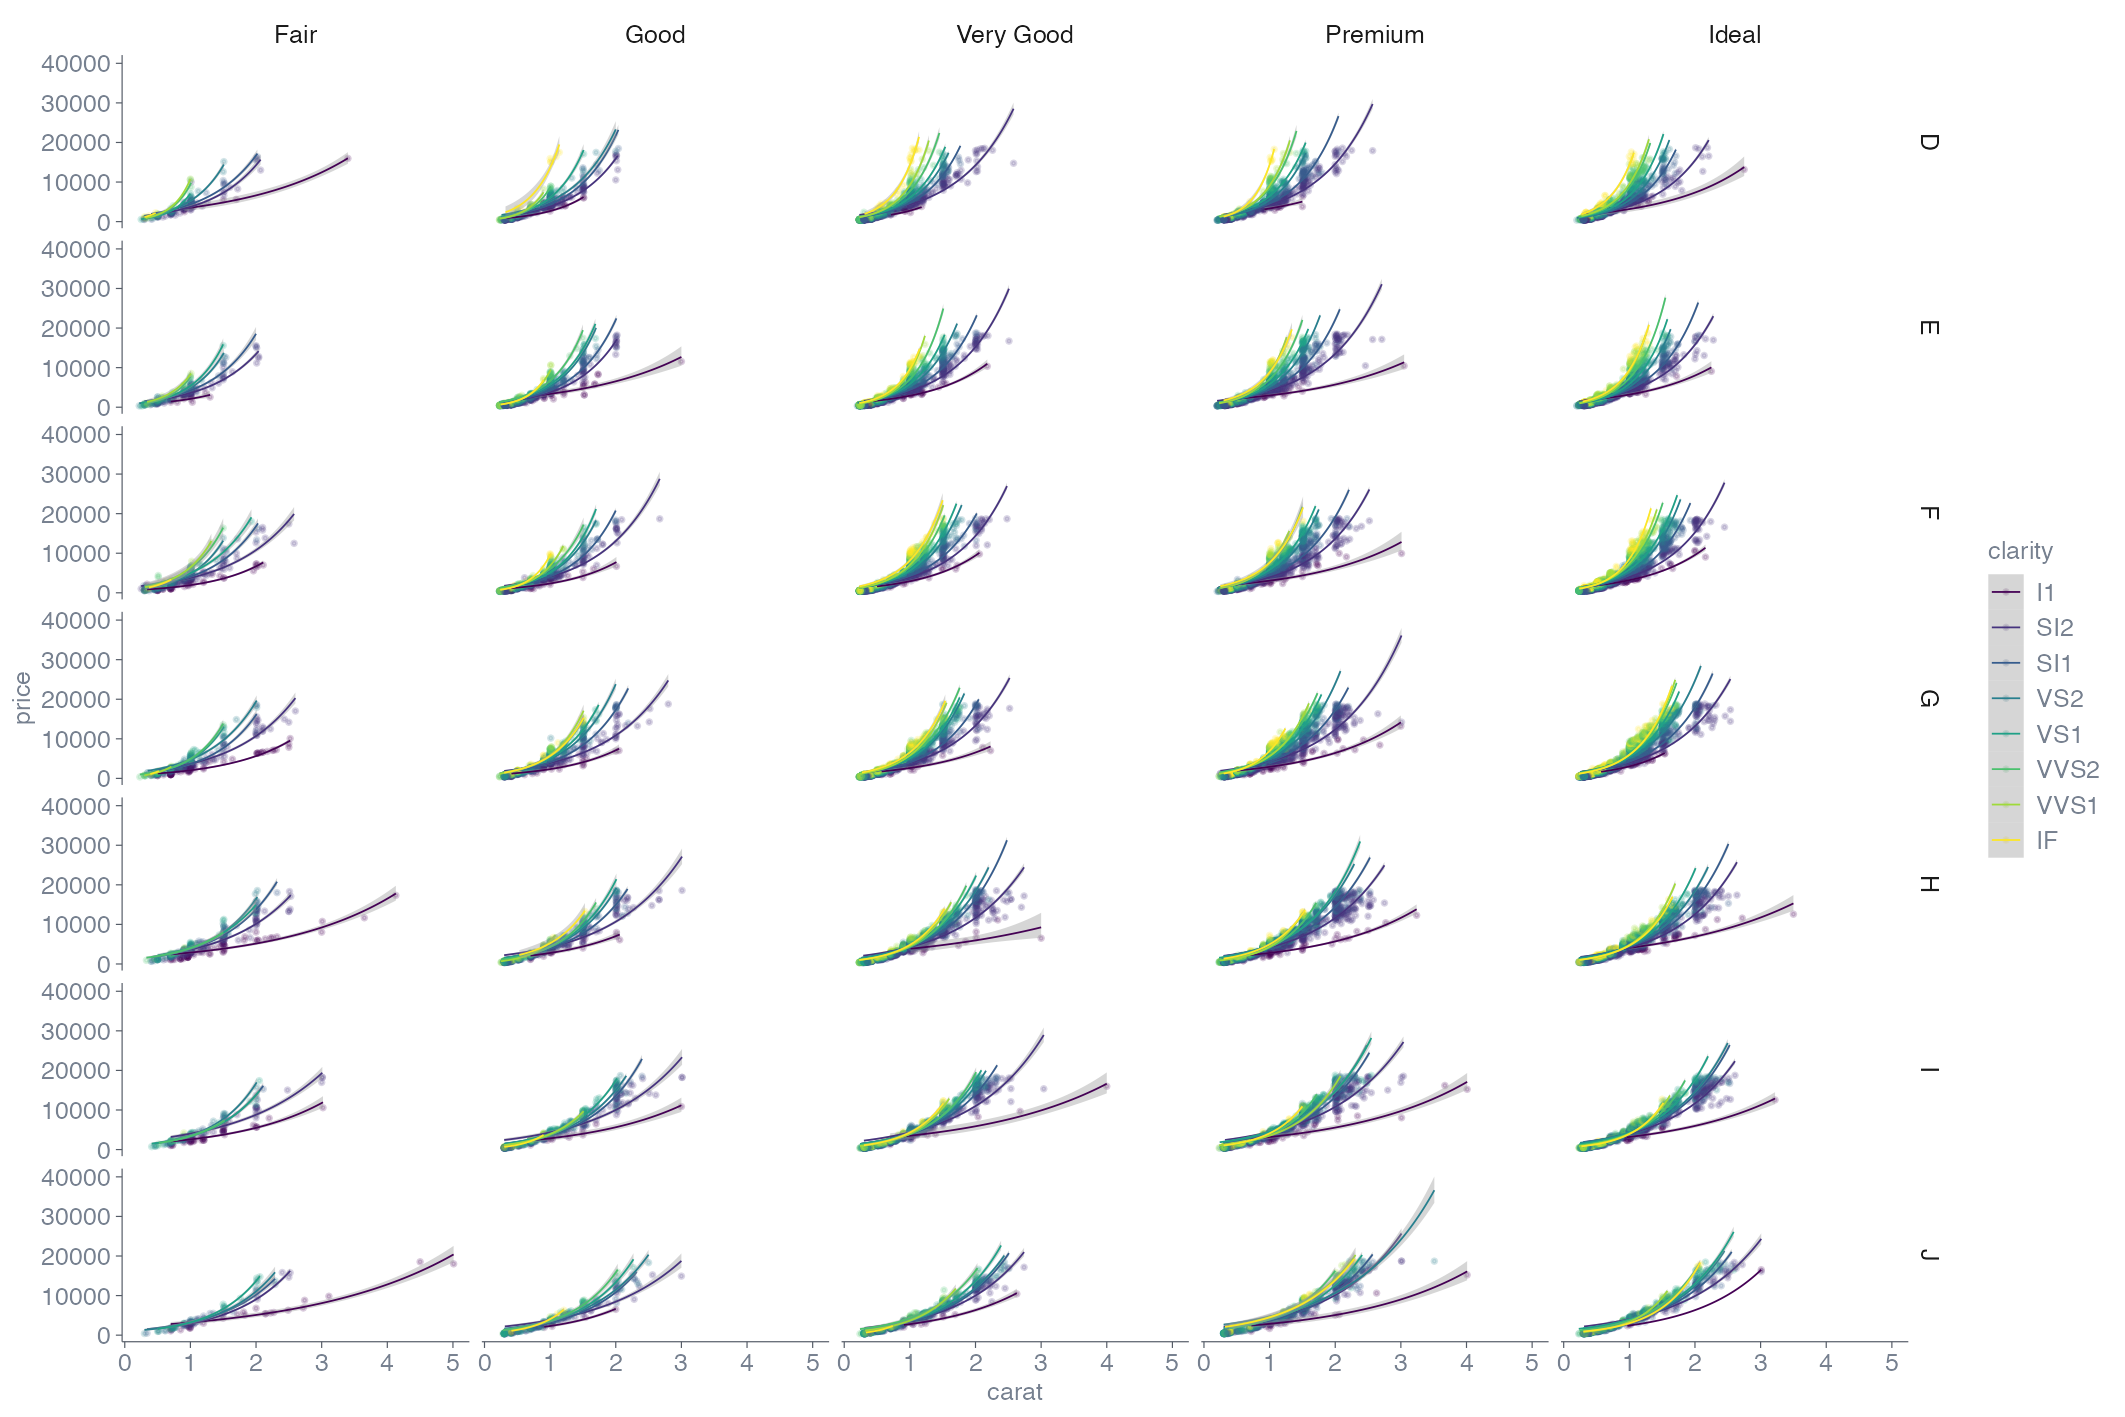
\includegraphics[width=\textwidth]{p_plot2}
    \caption{2カラムの横幅186 mmサイズの図の例。}
    \label{figure:figureExampleLarge}
\end{figure*}

\subsection*{表}

tabular環境を用いた標準的な表の例を表\ref{table:tableExample}に掲載する。

\begin{table}[hbt!]
 \caption{表の例}
 \label{table:tableExample}
 \centering
    \begin{tabular}{lllll}
        \toprule
        \multirow{2}{*}{Models} & \multicolumn{3}{c}{Metric 1} & Metric 2\\
        \cmidrule{2-4} \cmidrule{5-5} \\
        {} & precision & recall & F-score  & R@10 \\
        \midrule
        model 1 & 0.67  & 0.8 & 0.729  & 0.75 \\
        model 2 & 0.8 & 0.9 & 0.847 & 0.85 \\
        \bottomrule
    \end{tabular}
\end{table}

\subsection*{コードブロックとインラインコード}

コードブロックを挿入するには\verb|\verbatim|を用いるか、mintedパッケージを利用する。前述したように後者の利用にはPygmentsのインストールが必須である(Overleafには事前にインストールされているため不要)。以下にその例を示す。スクリプトの内容は、前述の図中の文字や軸の太さの節で推奨した設定を、R\cite{R_Core_Team2022-ar}の{tidyverse}\cite{Wickham2019-ex}ライブラリを用いてggplot2のテーマとして規定したものである。言語を設定するには\mintinline{latex}{\begin{minted}{language}}の\verb|language|部分を変更する。

\begin{minted}{r}
library(tidyverse)
theme_aiit <- 
  theme_minimal(6, base_family = "Helvetica") +
  theme(
    line = element_line(linewidth = .1/.75, colour = "#545B66"),
    text = element_text(size = 6, colour = "#778190"),
    title = element_text(size = 6, colour = "#778190"),
    panel.grid = element_blank(),
    axis.line = element_line(),
    axis.text = element_text(size = 6, colour = "#778190"),
    axis.ticks = element_line(),
    plot.background = element_rect(fill = "white", colour = NA),
    strip.text = element_text(size = 6),
    strip.switch.pad.grid = unit(2, "mm"),
    strip.placement = "outside",
    legend.text = element_text(size = 6),
    legend.key.size = unit(3, units = "mm"),
    plot.tag = element_text(
      size = 10, 
      family = "Helvetica", 
      face = "bold"
    )
  )
\end{minted}
このテーマで例に示した図\ref{figure:figureExample}をプロットするには、以下のようにする。
\begin{minted}{r}
iris |> 
  ggplot(
    aes(
      x = Sepal.Length, 
      y = Sepal.Width, 
      colour = Petal.Length, 
      group = Species)
  ) +
  geom_smooth(
    method = "lm", 
    size = .3/.75, 
    colour = "black", 
    fill = "grey80"
  ) +
  geom_point(size = .15/.75) +
  scale_x_continuous(breaks = 5:8) +
  scale_y_continuous(breaks = 2:4, labels = c(2, "", 4)) +
  scale_colour_viridis_c() +
  facet_wrap(vars(Species)) +
  theme_aiit +
  theme(legend.position = "bottom")
ggsave("./output/p_plot.png", width = 86, height = 60, unit ="mm", dpi = 600)
\end{minted}

同様に図\ref{figure:figureExampleLarge}をプロットするスクリプトは以下の通り。

\begin{minted}{r}
diamonds |> 
  ggplot(aes(carat, price, colour  = clarity)) +
  geom_point(size = .15/.75, alpha = .2) +
  geom_smooth(
    method = "glm", 
    method.args = list(family = gaussian(link = "log")),
    size = .2
  ) +
  facet_grid(cols = vars(cut), rows = vars(color)) +
  scale_colour_viridis_d() +
  theme_aiit
ggsave("./output/p_plot2.png", width = 180, height = 120, unit = "mm", dpi = 600)
\end{minted}

変数を本文中で言及する場合はたとえば\verb|\verb|を用いると\verb|date|となり、シンタックスハイライトを使いたい場合は\verb|\mintinline{language}{content}|を用いると\mintinline{r}{function(x) {x + 1}}となる。

\subsection*{数式}

数式の例を以下に示す。数式を参照するには\verb|\label|と\verb|\eqref|を使い、\eqref{eq:example}式のようにする。

\begin{equation}
\left( \int_0^\infty \frac{\sin x}{\sqrt{x}} dx \right)^2=
\sum_{k=0}^\infty \frac{(2k)!}{2^{2k}(k!)^2} \frac{1}{2k+1}=
\prod_{k=1}^\infty \frac{4k^2}{4k^2 -1}= \frac{\pi}{2} \label{eq:example}
\end{equation}

\begin{equation}
  c = 299{,}792{,}458 \, \mathrm{m/s}
\end{equation}

\begin{equation}
  A = \begin{pmatrix}
        a_{11} & \ldots & a_{1n} \\
        \vdots & \ddots & \vdots \\
        a_{m1} & \ldots & a_{mn}
      \end{pmatrix}
\end{equation}

\section{参考文献の引用}

本テンプレートの引用にはcitation-style-languageパッケージを用いているが、著者の責任においてbibtexやbiblatexなどを用いてもよい。本テンプレートファイルでは一例として、PaperPileを利用して参考文献を管理し、PaperPileのWork  flows and Integrations機能からOverleaf Integrationを選択したのち、発行されたURLを利用してオンラインのファイルを\verb|bibliography.bib|として接続している。設定は、Settings\textgreater BibTeX\textgreater Include identifiers (doi, pmid)とInclude URLsにチェックを入れ、Escape UTF-8 charactersとInclude abstractとInclude keywordsのチェックを外す。Zoteroの場合は、\href{https://github.com/zepinglee/citeproc-lua/issues/24}{citation-style-languageの開発者が推奨する}ように\href{https://retorque.re/zotero-better-bibtex/}{Better BibTeX}を使う方法がある(未検証)。

引用方式はPLOS形式を用いる。引用方式は\mintinline{latex}{\cslsetup{style=plos}}で指定済みである。\verb|style=plos|はフォルダに格納済みの\verb|plos.csl|に紐付けられているため、このファイルを削除したりしないこと。PLOS形式はヴァンクーヴァー形式のヴァリアントで、本文中での引用を(1)ではなく[1]に変更したものである。引用ルールの適用にはたとえばPLOS ONEウェブサイト\cite{Plos_undated-wc}からplos2015.bstファイルをダウンロードしてbibtex経由で適用してもよいが、ログファイルを経由しなければ一覧が生成できず煩雑なので、citation-style-languageパッケージの利用を推奨する。citation-style-languageパッケージにはアンダースコア(\verb|_|)を含むフィールドがあるとコンパイルが終わらない、\verb|howpublished={\url{}}|ではURLが表示されない、などの制限がある。そのため、コンパイルが終わらない際は.bibファイルのフォーマッティングに問題がある場合が多いので、面倒でも\mintinline{bib}{@comment{}}を使うなどして文献ごとに問題がないか、問題があるとすればどのフィールドなのかをチェックしていくことを推奨する。

日本語訳された書籍の例\cite{2019-yk}単著洋書の例\cite{Dawkins2006-fw, Dennett2017-xz}、単著英文論文の例\cite{Tehrani2013-dy}、共著英文論文の例\cite{Henrich2008-lq}、8人共著論文の例\cite{Cooney2017-yt}、共著和文論文の例\cite{2012-zr}、共著和書の例\cite{2012-dp}、共著和書の一章の例\cite{2017-dc}。これらはあくまで自動生成された例であるため、矛盾がある場合はPLOS ONEの引用形式\cite{Plos_undated-yh}に従うこと。

\section{その他}

\subsection*{紀要編集委員の例年のルーチンタスク}
\verb|variables.sty|内の変数を毎年更新する。
\subsection*{執筆の実例}

テンプレート更新の経緯についての紀要論文\cite{2024-oz}は2023年度版のLaTeXテンプレートを用いて執筆されている\cite{Matsui2023-px}。もし本LaTeXテンプレートを執筆に利用した方で、Overleafのプロジェクトを共有してもよい方はここにリストしたいのでShare projectから共有をオンにし、View権限のみのURLを紀要編集委員に提供いただきたい。
% 2025年度以降の紀要編集委員の方へ:プロジェクトのリストは引用ではなくここにURLをhref{Overleafへのリンク}{著者ら, yyyy}で羅列する想定です(管理が大変なので)。

\section{ライセンス}
著作権は著者に帰属する。クリエイティブ・コモンズ・ライセンスの表示が可能(表示しなくてもよい)。もし表示したい場合は、参考文献のあとに、\mintinline{latex}{\vspace{8mm}
\noindent

\includegraphics[height=8mm]{licenses/by}
\vspace{2mm}
\begin{spacing}{.6}
\noindent
\textbf{Open Access} This article is licensed under CC BY 4.0. To view a copy of this license, visit \url{https://creativecommons.org/licenses/by/4.0/}
\end{spacing}}のような形で羅列されたライセンスから適用したいバージョンを一つ選んで残し、他はコメントアウトするか削除する。もし表示したくない場合はすべてコメントアウトするか削除する。また、初回原稿提出時にGoogle Form上でライセンスを指定すること。このテンプレートファイルじたいのライセンスは表示 4.0 国際(CC BY 4.0)\cite{Creative_Commons_undated-dl}。

\printbibliography

% select an applicable license from the list below and comment out (or delete) the others
\vspace{8mm}
\noindent

\includegraphics[height=8mm]{licenses/by}
\vspace{2mm}
\begin{spacing}{.6}
\noindent
\textbf{Open Access} This article is licensed under CC BY 4.0. To view a copy of this license, visit \url{https://creativecommons.org/licenses/by/4.0/}
\end{spacing} 
% \vspace{8mm}
\noindent

\includegraphics[height=8mm]{licenses/by-sa}

\begin{spacing}{.6}
\noindent
\textbf{Open Access} This article is licensed under CC BY-SA 4.0. To view a copy of this license, visit \url{https://creativecommons.org/licenses/by-sa/4.0/}
\end{spacing} 
% \vspace{8mm}
\noindent

\includegraphics[height=8mm]{licenses/by-nd}

\begin{spacing}{.6}
\noindent
\textbf{Open Access} This article is licensed under CC BY-ND 4.0. To view a copy of this license, visit \url{https://creativecommons.org/licenses/by-nd/4.0/}
\end{spacing} 
% \vspace{8mm}
\noindent

\includegraphics[height=8mm]{licenses/by-nc}

\begin{spacing}{.6}
\noindent
\textbf{Open Access} This article is licensed under CC BY-NC 4.0. To view a copy of this license, visit \url{https://creativecommons.org/licenses/by-nc/4.0/}
\end{spacing} 
% \vspace{8mm}
\noindent

\includegraphics[height=8mm]{licenses/by-nc-sa}

\begin{spacing}{.6}
\noindent
\textbf{Open Access} This article is licensed under CC BY-NC-SA 4.0. To view a copy of this license, visit \url{https://creativecommons.org/licenses/by-nc-sa/4.0/}
\end{spacing} 
% \vspace{8mm}
\noindent

\includegraphics[height=8mm]{licenses/by-nc-nd}
\vspace{2mm}
\begin{spacing}{.6}
\noindent
\textbf{Open Access} This article is licensed under CC BY-NC-ND 4.0. To view a copy of this license, visit \url{https://creativecommons.org/licenses/by-nc-nd/4.0/}
\end{spacing} 


\end{document}
